\documentclass[tikz,border=0pt]{standalone}
\usepackage{amsmath, amssymb, bm}
\usetikzlibrary{positioning, arrows.meta, calc}

\begin{document}
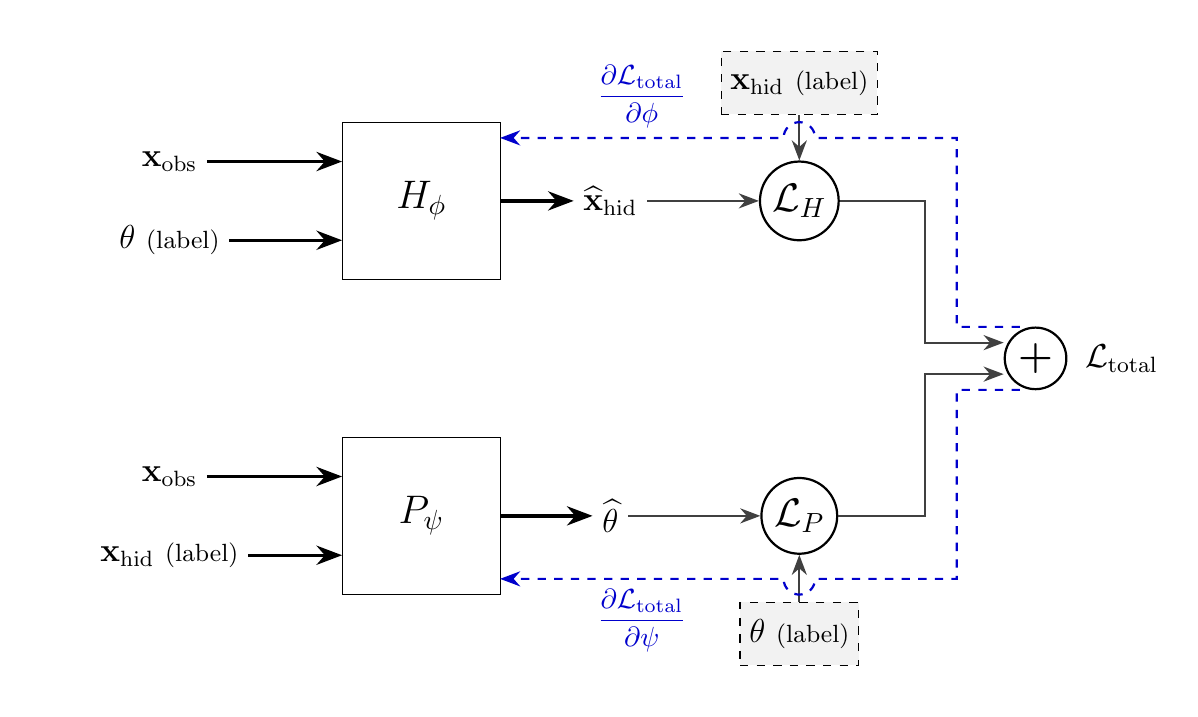
\begin{tikzpicture}[
    >={Stealth[scale=1.1]},
    netbox/.style={draw, rectangle, minimum width=2.0cm, minimum height=2.0cm, align=center, font=\Large, fill=white},
    txt/.style={align=center, font=\large},
    labelbox/.style={draw, dashed, rectangle, minimum width=1.5cm, minimum height=0.8cm, align=center, fill=gray!10, font=\large},
    lossnode/.style={draw, circle, inner sep=2pt, font=\Large, thick},
    mainarrow/.style={->, very thick, black},
    dataarrow/.style={->, thick, darkgray},
    backproparrow/.style={->, thick, dashed, blue!80!black}
]

% 두 그림의 크기와 기준점을 완벽히 일치시키는 강제 바운딩 박스

\useasboundingbox (-5.0, 2.2) rectangle (9.5, -6.2);

% H_phi Block & Inputs
\node[netbox] (H) at (0, 0) {$H_\phi$};
\node[txt] (u_H) at (-3.2, 0.5) {$\mathbf{x}_\mathrm{obs}$};
\node[txt] (theta_H) at (-3.2, -0.5) {$\theta$ \small{(label)}};
\draw[mainarrow] (u_H.east) -- (H.west |- u_H.east);
\draw[mainarrow] (theta_H.east) -- (H.west |- theta_H.east);

% Output & Loss
\node[txt] (xhat_H) at (2.4, 0) {$\widehat{\mathbf{x}}_{\mathrm{hid}}$};
\draw[mainarrow] (H.east) -- (xhat_H.west);
\node[lossnode] (LossH) at (4.8, 0) {$\mathcal{L}_H$};
\node[labelbox] (target_H) at (4.8, 1.5) {$\mathbf{x}_{\mathrm{hid}}$ \small{(label)}};
\draw[dataarrow] (xhat_H.east) -- (LossH.west);
\draw[dataarrow] (target_H.south) -- (LossH.north);

% P_psi Block & Inputs
\node[netbox] (P) at (0, -4.0) {$P_\psi$};
\node[txt] (u_P) at (-3.2, -3.5) {$\mathbf{x}_\mathrm{obs}$};
\node[txt] (xhid_P) at (-3.2, -4.5) {$\mathbf{x}_{\mathrm{hid}}$ \small{(label)}};
\draw[mainarrow] (u_P.east) -- (P.west |- u_P.east);
\draw[mainarrow] (xhid_P.east) -- (P.west |- xhid_P.east);

% Output & Loss
\node[txt] (thetahat_P) at (2.4, -4.0) {$\widehat{\theta}$};
\draw[mainarrow] (P.east) -- (thetahat_P.west);
\node[lossnode] (LossP) at (4.8, -4.0) {$\mathcal{L}_P$};
\node[labelbox] (target_P) at (4.8, -5.5) {$\theta$ \small{(label)}};
\draw[dataarrow] (thetahat_P.east) -- (LossP.west);
\draw[dataarrow] (target_P.north) -- (LossP.south);

% Total Loss
\node[draw, circle, inner sep=2pt, font=\Large, thick] (Sum) at (7.8, -2.0) {$\bm{+}$};
\node[txt, right=0.1cm of Sum] (L_total) {$\mathcal{L}_{\text{total}}$};
\draw[dataarrow] (LossH.east) -| (6.4, -1.8) -- (Sum.west |- 0,-1.8);
\draw[dataarrow] (LossP.east) -| (6.4, -2.2) -- (Sum.west |- 0,-2.2);

% Backpropagation
\draw[backproparrow] (7.6, -1.6) -| (6.8, 0.8) -- (5.0, 0.8) arc[start angle=0, end angle=180, radius=0.2cm] -- node[midway, above] {$\displaystyle \frac{\partial \mathcal{L}_{\mathrm{total}}}{\partial \phi}$} (1.0, 0.8);
\draw[backproparrow] (7.6, -2.4) -| (6.8, -4.8) -- (5.0, -4.8) arc[start angle=0, end angle=-180, radius=0.2cm] -- node[midway, below] {$\displaystyle \frac{\partial \mathcal{L}_{\mathrm{total}}}{\partial \psi}$} (1.0, -4.8);

\end{tikzpicture}
\end{document}